\RequirePackage[ngerman=ngerman-x-latest]{hyphsubst}

\documentclass[
    bibliography=totoc, cd=lightcolor, cdmath=false, ngerman]{tudscrreprt}

\usepackage[Algorithmus]{algorithm}
\usepackage{algpseudocode}
\usepackage{amsmath}
\usepackage{amssymb}
\usepackage{babel}
\usepackage{hyperref}
\usepackage[utf8]{inputenc}
\usepackage{listings}
\usepackage{pxfonts}
\usepackage[dvipsnames]{xcolor}

% import after xcolor to avoid clash
\usepackage{lstlinebgrd}

\lstset{
    basicstyle=\scriptsize,
    commentstyle=\color{Green}\bfseries,
    frame=single,
    framexleftmargin=3em,
    keywordstyle=\color{RoyalBlue}\bfseries,
    numbers=left,
    otherkeywords={size\_t, \#, \\, pragma, omp, parallel,
                   reduction, atomic, write, critical},
    xleftmargin=3em,
}

\begin{document}

\title{Komplexpraktikum Paralleles Rechnen}

\author{
  Timo Nicolai
  \course{Informationssystemtechnik}
  \matriculationnumber{4048209}
}

\supervisor{Dipl.-Ing. Oliver Knodel}

\headingsvskip=-100pt

\maketitle
\tableofcontents
\pagebreak

\chapter{Einleitung}
Dieser Beleg beschreibt die Implementierung von Lloyds k-means
Vektorquantisierungs-Algorithmus sowohl in serieller als auch parallelisierter
Form.

Die Parallelisierung wurde zum einen durch parallele Nutzung mehrerer CPU-Kerne
mittels OpenMP Quellcode-Annotationen und zum anderen durch Auslagern
parallelisierbarer Performance-kritischer Abschnitte auf eine NVIDIA-GPU
mittels CUDA erreicht. Beide Methoden werden im Folgenden mit Hinblick auf
Besonderheiten in der Implementierung und Performance-Gewinnen in Abhängigkeit
der Problem-Größe und genutzten Hardware-Ressourcen mit der seriellen
Implementierung gegenübergestellt.

\chapter{Der k-means Algorithmus}

\section{Beschreibung des Algorithmus}

Unter der Bezeichnung k-means sind mehrere Algorithmen bekannt, die alle zum
Ziel haben, auf effizientem Wege eine annähernde Lösung für das folgende Problem
zu finden:
\bigbreak
Eine Menge von Vektoren ist derart in $k$ Partitionen zu zerlegen, dass die
Summe der quadratischen euklidische Distanzen aller Vektoren in jeder Partition
zum jeweiligen Partitions-Schwerpunkt minimiert wird. D.h. sei $M$ eine Menge
von Vektoren $x \in \mathbb{R}^n$, dann sind Partitionen $P = \{P_i \mid i =
1,2,\dots,k\}$ von $M$ mit Schwerpunkten $S = \{\mu_i \mid i = 1, 2, \dots,
k\}$ gesucht, sodass der folgende Ausdruck minimal wird:
$$
\sum_{k} \sum_{x \in P_k} ||x - \mu_k||^2
$$
Der hier betrachtete Algorithmus ist wohl der bekannteste und einfachste unter
diesen Algorithmen und wurde erstmals von Lloyd vorgeschlagen \cite{bib:lloyd}.
Er basiert auf der wiederholten Zuweisung von Vektoren zu den Partitionen mit
den ihnen am nähsten gelegenen Schwerpunkten und folgender Neuberechnung dieser
Schwerpunkte und ist in Algorithmus~\ref{alg:lloyd} dargestellt.

\begin{algorithm}
    \caption{Llyods k-means Algorithmus}
    \begin{algorithmic}[1]
        \Procedure{k-means}{$x$}
            \State // Initialisiere Schwerpunkte mit zufälligen Vektoren
            \For{$i = 1 \dots k$}
                \State $P_i := \emptyset$
                \State $\mu_i := \text{ein zufälliges } x_j \in M$
            \EndFor
            \State // Berechne (annähernd) ideale Partitionen iterativ
            \While{Änderungen an $P$} \label{alg:loop_begin}
                \State // Weise Vektoren den Partitionen mit nächstem Schwerpunkt zu
                \For{$x_i \in M$} \label{alg:cluster_begin}
                    \State $j := \mathrm{argmin}_j\ ||x_i - \mu_j||$
                    \State $P_j := P_j \cup \{x_i\}$
                \EndFor \label{alg:cluster_end}
                \State // Aktualisiere Partitions-Schwerpunkte
                \For{$i = 1 \dots k$}
                    \State $\mu_i := |P_i|^{-1} \sum_{x_j \in P_i} x_j$
                \EndFor
            \EndWhile \label{alg:loop_end}
        \EndProcedure
    \end{algorithmic}
    \label{alg:lloyd}
\end{algorithm}

Es ist zusätzlich zu beachten, dass es mehrere denkbare Bedingungen für den den
Abbruch der Schleife in den Zeilen \ref{alg:loop_begin} bis \ref{alg:loop_end}
geben kann. Die in Algorithmus~\ref{alg:lloyd} gezeigte triviale
Abbruchbedingung greift dann, wenn in einer Iteration kein Vektor die Partition
wechselt. In diesem Fall wurde eine stationäre Lösung gefunden uns die
Berechnung kann abgebrochen werden. Auch möglich ist es, von vorneherein ein
Limit für die Anzahl der Iterationen festzulegen nach welchem abgebrochen wird
auch wenn kein stationäre Lösung gefunden wurde. Eine weitere Möglichkeit wäre
es, dann abzubrechen wenn sich in einer Iteration keiner der
Partitions-Schwerpunkte um mehr als einen Schwellwert $\epsilon$ von seinem
vorherigen Wert entfernt. In den folgenden Implementierungen wird stets mit
einem Iterations-Limit von 100 gearbeitet (das praktischen Untersuchungen nach
jedoch selten erreicht wird).

Außerdem ist in Algorithmus~\ref{alg:lloyd} die Behandlung leer verbliebener
Partitionen nach der Schleife in den Zeilen \ref{alg:cluster_begin} bis
\ref{alg:cluster_end} nicht dargestellt. Dieser Fall sollte in einer
``vernünftigen'' Implementierung eher die Ausnahme als die Regel darstellen,
muss aber trotzdem behandelt werden um die Korrektheit des Algorithmus zu
garantieren. Der in den folgenden Implementierungen gewählte Ansatz ist es,
iterativ alle leere Partitionen mit dem Vektor aus der jeweils momentan größten
Partition, der von deren Schwerpunkt am weitesten entfernt ist, zu füllen.

Der Algorithmus kann wie er hier dargestellt ist, Mengen von Vektoren beliebiger
Dimensionen angewandt werden. Im Folgenden wird allerdings nur noch die Anwendung
des k-means Algorithmus zur Segementierung von Farbbildern betrachtet (und
somit der Fall $x \in F \subset \mathbb{R}^3$ unter der Annahme, dass $M$ die
Menge aller Pixel eines Bildes in \texttt{RGB}-Vektordarstellung und $F$ der
\texttt{RGB}-Farbraum ist, d.h. $x = (r, g, b)^T$ mit $r, g, b \in [0,
255])$.

\section{Sequentielle Implementierung}

\subsubsection{Aufruf}

Quelltext~\ref{lst:kmeansc} zeigt eine sequentielle Implementierung des k-means
Algorithmus in C. Die Funktion \texttt{kmeans} in Zeile 30 zerlegt die in
\texttt{n\_pixels} in \texttt{pixels} gespeicherten Pixel in
\texttt{n\_centroids} Partitionen mit den Schwerpunkten \texttt{centroids}. Die
Funktion weist zu diesem Zweck jedem Pixel \texttt{pixels[i]} in
\texttt{labels[i]} den Index der Partition zu der dieser Pixel gehört zu.
\texttt{struct pixel} repräsentiert dabei einen Punkt im \texttt{RGB}-Farbraum
und ist wie in Quelltext~\ref{lst:structpixel} gezeigt definiert.

\lstinputlisting[language=C, firstline=4, lastline=7,
caption={\texttt{struct pixel}}, label=lst:structpixel]{../../c/include/kmeans.h}

Will man die Funktion nutzen um ein Farbbild zu segmentieren, muss man also
zunächst die Pixel des Bildes in ein eindimensionales Array vom Typ
\texttt{struct pixel[]} transformieren und der Funktion \texttt{kmeans}
übergeben. Anschließend kann dann der jeweils i-te Pixel durch den in
\texttt{centroids[labels[i]]} gespeicherten Schwerpunkt der Partitionen der er
zugeteilt wurde ersetzt und anschließend das zweidimensionale Bild
rekonstruiert werden.

\subsubsection{Ablauf}

In den Zeilen 42-49 findet die zufällige Initialisierung der
Partitions-Schwerpunkte statt. Die Hauptschleife in den Zeilen 52-153 iteriert
solange, bis keine Neuverteilung von Pixeln auf Partitionen mehr stattfindet
oder \texttt{KMEANS\_MAX\_ITER} Iterationen erreicht worden sind. Dabei werden
in den Zeilen 56-78 alle Pixel den Partitionen mit dem ihnen am nächsten
liegenden Schwerpunkt zugewiesen. Gleichzeitig werden die Summen aller Pixel in
jeder Partition im Array \texttt{sums} und die Größen der Partitionen im Array
\texttt{counts} festgehalten. In den Zeilen 81-131 wird die (verhältnismäßig
aufwändige aber in den meisten Anwendungsfällen selten auftretende)
Umverteilung von Pixeln auf eventuell leer gebliebene Partitionen vorgenommen.
In Zeilen 134-148 werden die neuen Schwerpunkte über die in \texttt{sums} und
\texttt{counts} gepeicherten Werte berechnet.

TODO: profiling

\lstinputlisting[language=C, firstline=10, lastline=163,
caption={Iterative k-means Implementierung in C},
label=lst:kmeansc]{../../c/src/kmeans.c}

\chapter{Parallelisierung}
\section{OpenMP}
Quelltext~\ref{lst:kmeansomp} zeigt die mittels OpenMP parallelisierte Variante
der in Quelltext~\ref{lst:kmeansc} gezeigten C-Implementierung. Modifizierte
Zeilen sind farbig hervorgehoben. Es mussten nur einige wenige Änderungen
vorgenommen werden um eine performante Parallelisierung zu erreichen, hier
zeigt sich eine große Stärke von OpenMP: existierender Code kann teilweise
(fast) ohne Änderungen am Code selbst nur durch die Nutzung von
\texttt{\#pragma} Direktiven parallelisiert werden.  Natürlich muss für
maximale Ausnutzung der dem Algortihmus inhärenten Parallelisierbarkeit eine
geeignete Code-Struktur vorliegen, dies ist hier aber prinzipiell bereits
gegeben, da die Performance-kritische Schleife in Zeilen 56-78 in
Quelltext~\ref{lst:kmeansc} bereits in geigneter Form gegeben ist.

\lstinputlisting[language=C, firstline=165, lastline=296,
caption={Parallilisierte k-means Implementierung mit OpenMP},
label=lst:kmeansomp,
linebackgroundcolor={%
    \ifnum\value{lstnumber}=9\color{yellow}\fi
    \ifnum\value{lstnumber}=16\color{yellow}\fi
    \ifnum\value{lstnumber}=17\color{yellow}\fi
    \ifnum\value{lstnumber}=27\color{yellow}\fi
    \ifnum\value{lstnumber}=28\color{yellow}\fi
    \ifnum\value{lstnumber}=40\color{yellow}\fi
    \ifnum\value{lstnumber}=45\color{yellow}\fi
    \ifnum\value{lstnumber}=46\color{yellow}\fi
    \ifnum\value{lstnumber}=47\color{yellow}\fi
    \ifnum\value{lstnumber}=48\color{yellow}\fi
    \ifnum\value{lstnumber}=77\color{yellow}\fi
    \ifnum\value{lstnumber}=84\color{yellow}\fi
    \ifnum\value{lstnumber}=85\color{yellow}\fi
    \ifnum\value{lstnumber}=90\color{yellow}\fi
    \ifnum\value{lstnumber}=99\color{yellow}\fi
    \ifnum\value{lstnumber}=100\color{yellow}\fi
    \ifnum\value{lstnumber}=101\color{yellow}\fi
    \ifnum\value{lstnumber}=102\color{yellow}\fi
    \ifnum\value{lstnumber}=104\color{yellow}\fi
    \ifnum\value{lstnumber}=105\color{yellow}\fi
    \ifnum\value{lstnumber}=106\color{yellow}\fi
    \ifnum\value{lstnumber}=107\color{yellow}\fi
    \ifnum\value{lstnumber}=117\color{yellow}\fi
    \ifnum\value{lstnumber}=120\color{yellow}\fi
    \ifnum\value{lstnumber}=121\color{yellow}\fi
    \ifnum\value{lstnumber}=122\color{yellow}\fi
    \ifnum\value{lstnumber}=124\color{yellow}\fi}]{../../c/src/kmeans.c}

Hier können die Berechnungen für jeden Pixel unabhängig voneinander erfolgen,
es muss lediglich der Zugriff auf die gemeinsamen Variable \texttt{done},
\texttt{sums} und \texttt{counts} synchronisiert werden. Für erstere genügt
eine \texttt{\#pragma atomic write} Direktive, für die beiden Arrays kann die
\texttt{reduction} Klausel \footnote{Seit OpenMP Version 4.5 (z.B. von GCC ab
Version 6.1 unterstützt) auf Arrays anwendbar.} genutzt werden. Hierbei muss
dann allerdings auch \texttt{sums} in ein Array von Fließkommazahlen
umgewandelt werden (jeweils drei aufeinander folgende ersetzen ein
\texttt{struct pixel}) um die Reduktion zu ermöglichen.

Andere Abschnitte des Algorithmus können potentiell ebenfall parallelisiert
werden, allerdings mit vergleichbar kleinem Performance-Gewinn. Bei der
Reparatur leerer Partitionen wurde ebenfalls über die einzelnen Pixel
parallelisiert, dieser Codeabschnitt wird jedoch nur selten (wenn überhaupt)
aufgerufen. Eine Parallelisierung über die Schwerpunkte (z.B. in Zeilen 134-148
in Quellcode~\ref{lst:kmeansc} lohnt sich aufgrund der in realistischen
Anwendungsfällen im Vergleich zur Anzahl der Pixel kleinen Zahl der Partitionen
nicht.

\section{CUDA}

\chapter{Nutzung des Repositorys}

\section{Demo}

Wird aus dem Wurzelverzeichnis des Repositorys \texttt{make demo} ausgeführt,
werden die verschiedenen Implementierungen auf das Beispiel-Bild
\texttt{images/demo\_image.jpg} angewandt und die Ergebnisse dargestellt. Da
die initialen Partitions-Schwerpunkte zufällig gewählt werden kann es unter
Umständen vorkommen, dass die Ergebnisse leicht unterschiedlich ausfallen
(auch in Abhängigkeit der maximalen Anzahl von Iterationen).
Abbildung~\ref{img:demoresults} zeigt ein Beispiel

\begin{figure}[h]
\centering
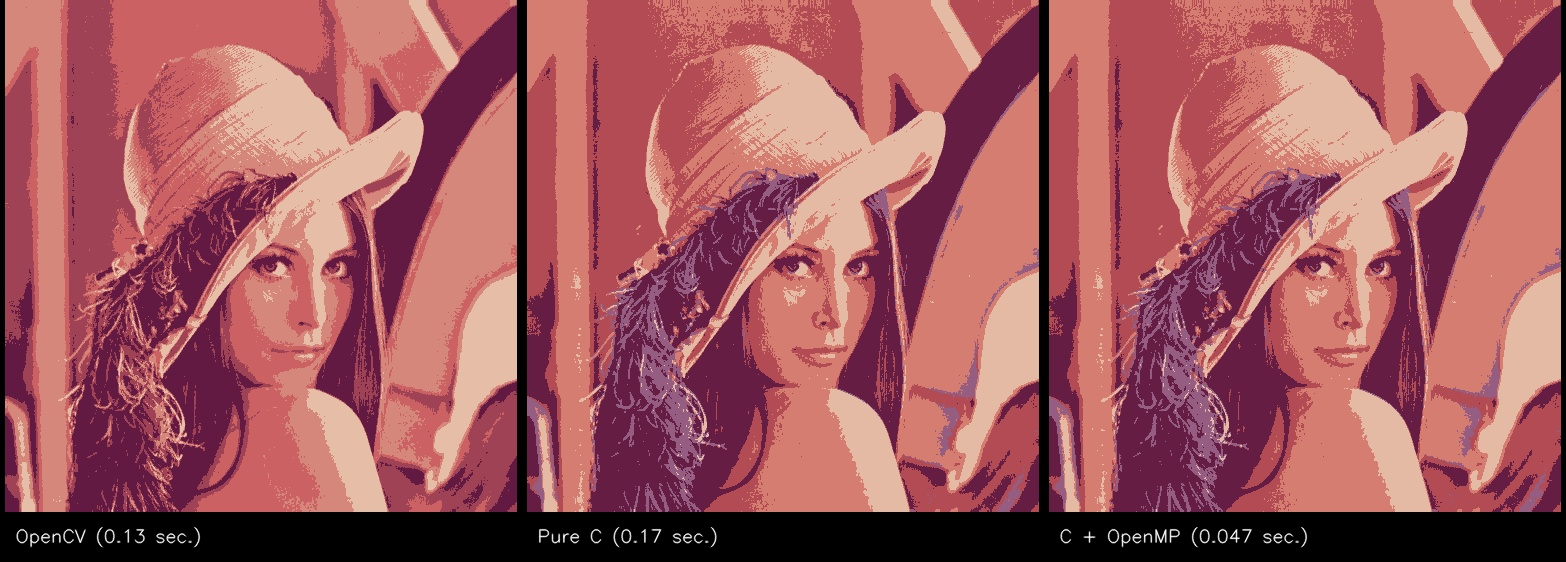
\includegraphics[width=\textwidth]{report/resources/demo_results.jpg}
\caption{Beispielhafte Demo Ergebnisse}
\label{img:demoresults}
\end{figure}

\section{Benchmark}

Bei Ausführung von \texttt{make benchmark} werden die Implementierungen
hingegen entsprechend der im \texttt{Makefile} gesetzten Parameter auf zufällig
generierte Bilder verschiedener Größen mit variierenden Partitions-Größen
angewandt und jeweils die Ausführungszeiten in \texttt{.csv} Datein im
\texttt{benchmarks} Verzeichnis protokolliert. Mit dem Python script
\texttt{tool/plot} können die Ergbenisse visualisiert werden, dazu muss
\texttt{./tool/plot benchmarks} ausgerufen werden (passiert bei Ausführung von
\texttt{make benchmark} automatisch).

\chapter{Quellcode}

\begin{thebibliography}{1}
\bibitem[1]{bib:lloyd}
Lloyd., S. P. (1982). ``Least squares quantization in PCM''. IEEE Transactions
on Information Theory
\end{thebibliography}

\end{document}
